% !TEX program = arara
% arara: pdflatex
% arara: biber
% arara: pdflatex
% arara: pdflatex
% arara: clean: { files: [ Paper.out ] }
% arara: clean: { files: [ Paper.aux, Paper.bbl ] }
% arara: clean: { files: [ Paper.bcf, Paper.blg ] }
% arara: clean: { files: [ Paper.log, Paper.run.xml ] }
% arara: clean: { files: [ Paper.toc, Paper-blx.bib ] }
% 

\documentclass{Paper}
\usepackage{ngerman}
\usepackage[utf8]{inputenc}
\usepackage{todonotes}
\usepackage{xcolor}
\usepackage{tikz}
\usepackage{pgf-pie}
\usepackage{pgfplots}
\usepackage{hyperref} % http://ctan.org/pkg/hyperref
\hypersetup{
	colorlinks = true,
	linkcolor  = black
}

% define custom colours
\definecolor{greenOfApproval}{HTML}{009933}
\definecolor{redOfDisapproval}{HTML}{cc0000}
\definecolor{yellowOfBrevity}{HTML}{ffcc66}
\definecolor{purpleOfLengthiness}{HTML}{6600cc}


\begin{document}

\maketitle

% % % % %

\tableofcontents
\clearpage
	
\section{Abstrakt}
\todo[inline]{Autor: Berna}
	Yo
	
\section{Einleitung}
\todo[inline]{Autor: Kim}
	Yo
	
\section{Methode}
	\todo[inline]{Autor: Nizan \& Alina}
	\subsection{Versuchspersonen}
	\subsection{Apparaturen}
	\subsection{Prozedur}
	\subsection{Begründung des Aufbaus der Szenarien}
	\subsection{Begründung der Wartezeit \& Abschätzungen}
	\subsection{Methodik der Auswertung}
	
\section{Ergebnisse}
	\todo[inline]{Autor: Jana \& Chovi (\& Nicole \& Svenja)}


	SCATTERPLOTS ohne Gespräch
	\textit{axen und echte daten anpassen. verschiedene daten mit untersch. farben eintragen. u.u. minipages einrichten und seitenformatierung ändern}

	\begin{tikzpicture}
	\begin{axis}[%
	scatter/classes={%
	    a={mark=o,draw=black}},
	    axis lines=middle,
	    axis line style={->},
	    x label style={at={(axis description cs:0.5,-0.1)},anchor=north},
	    y label style={at={(axis description cs:-0.1,.5)},rotate=90,anchor=south},
	    xlabel={Alter},
	    ylabel={Zeiteinschätzung}]
	    
	    \addplot[scatter,only marks,%
	    scatter src=explicit symbolic]%
	table[meta=label] {
	x y label
	18 4.3 a
	80 5.1 a

	    };
	  
	\end{axis}
	\end{tikzpicture}



	\begin{tikzpicture}
	\begin{axis}[%
	scatter/classes={%
	    a={mark=o,draw=black}},
	    axis lines=middle,
	    axis line style={->},
	    x label style={at={(axis description cs:0.5,-0.1)},anchor=north},
	    y label style={at={(axis description cs:-0.1,.5)},rotate=90,anchor=south},
	    xlabel={Intelligenz},
	    ylabel={Zeiteinschätzung}]
	    
	    \addplot[scatter,only marks,%
	    scatter src=explicit symbolic]%
	table[meta=label] {
	x y label
	18 4.3 a
	80 5.1 a

	    };
	  
	\end{axis}
	\end{tikzpicture}


	\begin{tikzpicture}
	\begin{axis}[%
	scatter/classes={%
	    a={mark=o,draw=black}},
	    axis lines=middle,
	    axis line style={->},
	    x label style={at={(axis description cs:0.5,-0.1)},anchor=north},
	    y label style={at={(axis description cs:-0.1,.5)},rotate=90,anchor=south},
	    xlabel={Temperatur},
	    ylabel={Zeiteinschätzung}]
	    
	    \addplot[scatter,only marks,%
	    scatter src=explicit symbolic]%
	table[meta=label] {
	x y label
	18 4.3 a
	80 5.1 a

	    };
	  
	\end{axis}
	\end{tikzpicture}

	SCATTERPLOTS mit Gespräch 
	\textit{tatsächliche daten eintragen, axen anpassen}


	\begin{tikzpicture}
	\begin{axis}[%
	scatter/classes={%
	    a={mark=o,draw=black}},
	    axis lines=middle,
	    axis line style={->},
	    x label style={at={(axis description cs:0.5,-0.1)},anchor=north},
	    y label style={at={(axis description cs:-0.1,.5)},rotate=90,anchor=south},
	    xlabel={Alter},
	    ylabel={Zeiteinschätzung}]
	    
	    \addplot[scatter,only marks,%
	    scatter src=explicit symbolic]%
	table[meta=label] {
	x y label
	18 4.3 a
	80 5.1 a

	    };
	  
	\end{axis}
	\end{tikzpicture}



	\begin{tikzpicture}
	\begin{axis}[%
	scatter/classes={%
	    a={mark=o,draw=black}},
	    axis lines=middle,
	    axis line style={->},
	    x label style={at={(axis description cs:0.5,-0.1)},anchor=north},
	    y label style={at={(axis description cs:-0.1,.5)},rotate=90,anchor=south},
	    xlabel={Intelligenz},
	    ylabel={Zeiteinschätzung}]
	    
	    \addplot[scatter,only marks,%
	    scatter src=explicit symbolic]%
	table[meta=label] {
	x y label
	18 4.3 a
	80 5.1 a

	    };
	  
	\end{axis}
	\end{tikzpicture}


	\begin{tikzpicture}
	\begin{axis}[%
	scatter/classes={%
	    a={mark=o,draw=black}},
	    axis lines=middle,
	    axis line style={->},
	    x label style={at={(axis description cs:0.5,-0.1)},anchor=north},
	    y label style={at={(axis description cs:-0.1,.5)},rotate=90,anchor=south},
	    xlabel={Temperatur},
	    ylabel={Zeiteinschätzung}]
	    
	    \addplot[scatter,only marks,%
	    scatter src=explicit symbolic]%
	table[meta=label] {
	x y label
	18 4.3 a
	80 5.1 a

	    };
	  
	\end{axis}
	\end{tikzpicture}



	- ,,Hatten Sie Spaß?'' $<=>$ Zeitwahrnehmung  ? 
	\begin{figure}[ht]
	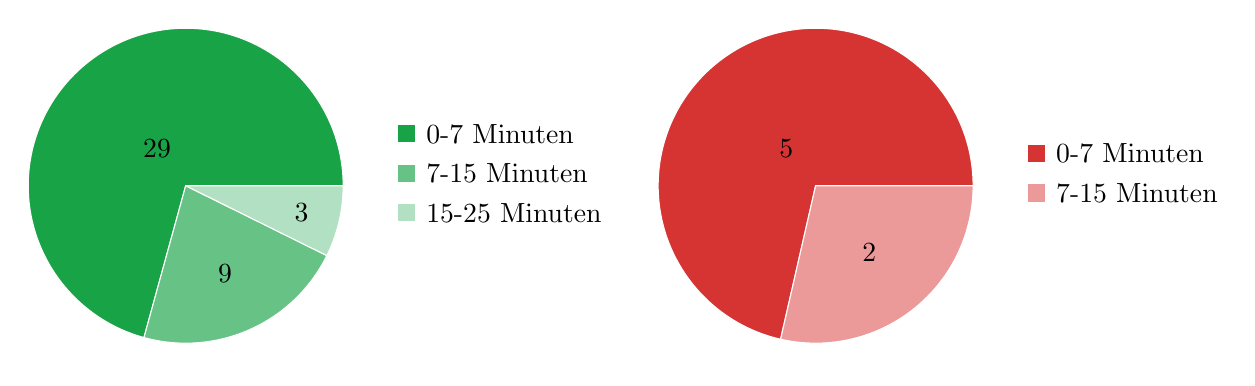
\begin{tikzpicture}
	\tikzset{lines/.style={draw=white},}
	\pie[color={greenOfApproval!90, greenOfApproval!60, greenOfApproval!30},radius = 2 ,sum=auto, after number=,text=legend,every only number node/.style={text=black},style={lines}]{29/0-7 Minuten,9/7-15 Minuten,3/15-25 Minuten}


	\tikzset{lines/.style={draw=white},}
	\pie[pos={8,0},radius = 2, color={redOfDisapproval!80, redOfDisapproval!40},sum=auto, after number=,text=legend,every only number node/.style={text=black},style={lines}]{5/0-7 Minuten,2/7-15 Minuten}
	\end{tikzpicture}
	\caption{Links: hatten Spaß. Rechts: hatten \textit{keinen} Spaß}
	\end{figure}

		
	- Szenarien sortieren kurz $->$ lang

	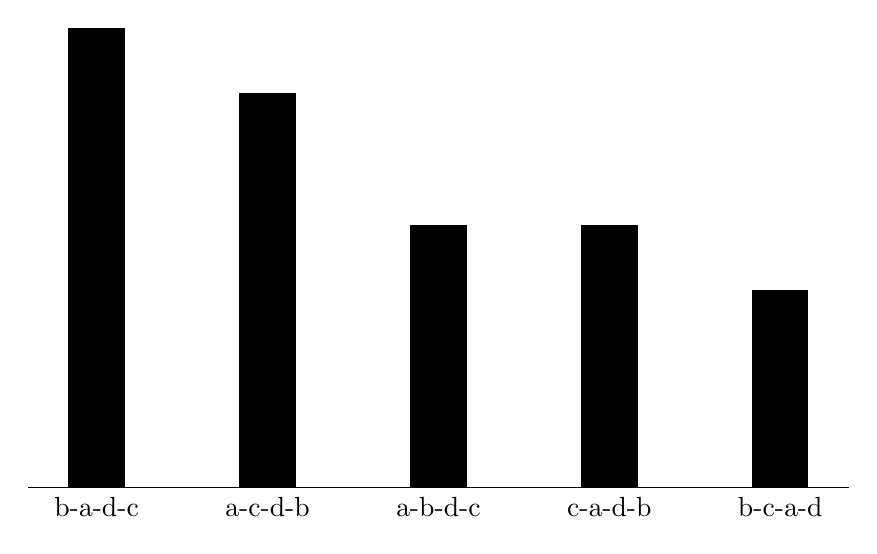
\begin{tikzpicture}
	\begin{axis}[
	     width  = 12cm,
	     hide y axis,
	     axis x line*=bottom,
	     height = 8cm,
	    bar width=20pt,
	     symbolic x coords={b-a-d-c, a-c-d-b, a-b-d-c, c-a-d-b, b-c-a-d},
	     %nodes near coords,
	     ymin=0,
	     xtick=data
	     ]
	     
	     
	     \addplot[ybar, fill=black] coordinates {
	          (b-a-d-c,7)
	          (a-c-d-b,6)
	          (a-b-d-c,4)
	          (c-a-d-b,4)
	          (b-c-a-d,3)
	     };
	\end{axis}
	\end{tikzpicture}

	Oben zu sehen: die Anzahl der Probanden, die die Szenarien entsprechend von kurz nach lang sortiert haben. D.h. konkret, dass insgesamt sieben Probanden   \textbf{b} für das kürzeste Szenario hielten und dann aufsteigend über \textbf{a} und \textbf{d} nach  \textbf{c} sortiert haben. \\
	Sechs Probanden waren der Ansicht, \textbf{a} sei das kürzeste Szenario gewesen, gefolgt von \textbf{c}, \textbf{d} und schließlich \textbf{b}. 

	weitere werte: s. zettel

	\textit{an den balken fehlen die zahlen}

		
	Aus diesen Daten kann man herleiten, wie viele Personen ein Szenario als das kürzeste (Diagramm in gelb) bzw. längste (Diagramm in lila) empfunden haben. 

	\begin{figure}[ht]
	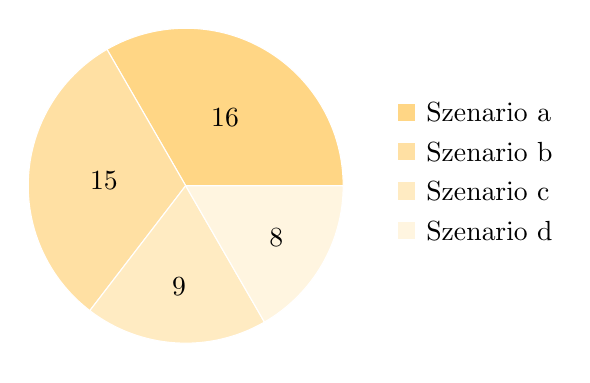
\begin{tikzpicture}
	\tikzset{lines/.style={draw=white},}
	\pie[color={yellowOfBrevity!80, yellowOfBrevity!60, yellowOfBrevity!40, yellowOfBrevity!20},radius = 2 ,sum=auto, after number=,text=legend,every only number node/.style={text=black},style={lines}]{16/Szenario a,15/Szenario b,9/Szenario c, 8/Szenario d}
	\end{tikzpicture}
	\caption{Welches Szenario war das kürzeste?}
	\end{figure}
		
	Von allen Probanden haben 15 angegeben Szenario \textbf{a} als das kürzeste empfunden zu haben, knapp dahinter steht Szenario \textbf{b} mit 14 Stimmen. Im Vergleich dazu sind die Szenarien \textbf{c} und \textbf{d} mit 9 und 8 Stimmen etwas abgeschlagen. Eine eindeutige Mehrheit gibt es dennoch nicht.\\
	Gleichermaßen kann man feststellen, welches Szenario von den meisten Personen als das längste bewertet wurde:

	\begin{figure}[ht]
	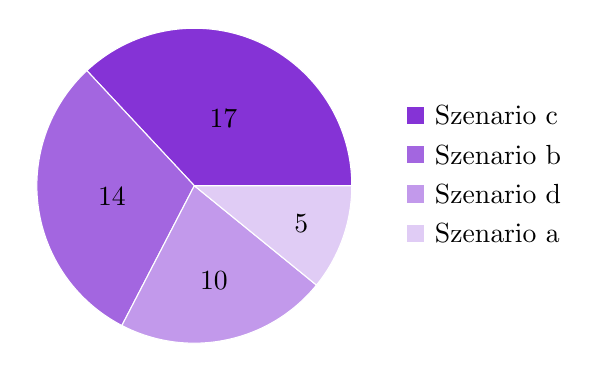
\begin{tikzpicture}
	\tikzset{lines/.style={draw=white},}
	\pie[color={purpleOfLengthiness!80, purpleOfLengthiness!60, purpleOfLengthiness!40, purpleOfLengthiness!20},radius = 2 ,sum=auto, after number=,text=legend,every only number node/.style={text=black},style={lines}]{17/Szenario c,14/Szenario b,10/Szenario d, 5/Szenario a}
	\end{tikzpicture}
	\caption{Welches Szenario war das längste?}
	\end{figure}	

	Auch bei der Bewertung des \textit{längsten} Szenarios gibt es keine ganz klare Mehrheit, dennoch heben sich zwei Szenarien etwas ab. 17 Probanden sind der Meinung, Szenario \textbf{c} sei das längste gewesen, danach kommen die Szenarien \textbf{b} mit 14 Stimmen und \textbf{d} mit 10 Stimmen. Abgeschlagen zum Schluss wird Szenario \textbf{a} mit nur 5 Stimmen genannt.\\
	Auffällig ist, dass es keine einheitliche Meinung gibt, welches Szenario das längste oder kürzeste ist, allerdings zeichnen sich ein paar Tendenzen ab. So ist sich die relative Mehrheit der Probanden sicher, \textbf{a} sei das längste Szenario und dementsprechend wenige behaupten das direkte Gegenteil. Ähnlich verhält es sich bei Szenario \textbf{c}, welches im auch verhältnismäßig oft als das längste bewertet wurde und nur sehr wenig als das kürzeste.\\
	Auffällig ist allerdings auch, dass die Meinungen bei \textbf{b} recht stark auseinandergehen. Ein Großteil der Befragten sieht dieses Szenario entweder als das längste oder als das kürzeste an, es gibt nur wenig Verteilung im Mittelbereich.
		
		
		
		
	\textit{korrelieren gutundschlecht und schnellundlangsam? im folgenden diese und jene diagramme etc pp}


		
		
		Die Probanden wurden darum gebeten, die vier erlebten Szenarien ebenfalls von \textit{gut} nach \textit{schlecht} zu sortieren. Nach unserer Hypothese (HIER HYPOTHESE EINFÜGEN),  


	\textit{TODO drei probandenzahlen fehlen noch. text und diagramme beizeiten anpassen\\
	TODO einheitliche zeitform}

		\begin{figure}[ht]
	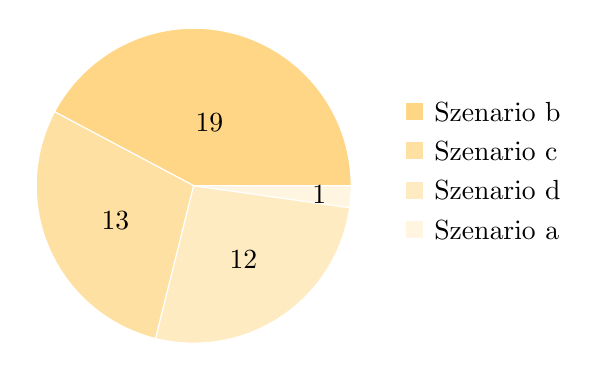
\begin{tikzpicture}
	\tikzset{lines/.style={draw=white},}
	\pie[color={yellowOfBrevity!80, yellowOfBrevity!60, yellowOfBrevity!40, yellowOfBrevity!20},radius = 2 ,sum=auto, after number=,text=legend,every only number node/.style={text=black},style={lines}]{19/Szenario b,13/Szenario c,12/Szenario d, 1/Szenario a}
	\end{tikzpicture}
	\caption{Welches war das beste Szenario?}
	\end{figure}

	Die Mehrheit der Probanden stimmt mit 19 Stimmen für Szenario \textbf{b} als das beste. \textbf{c} und darauffolgend \textbf{d} liegen im Mittelfeld. Weit abgeschlagen mit nur einer Stimme steht Szenario \textbf{a} auf dem letzten Platz.
		
		
		\begin{figure}[ht]
	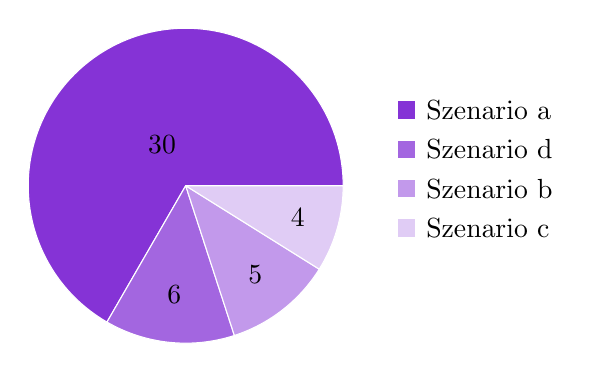
\begin{tikzpicture}
	\tikzset{lines/.style={draw=white},}
	\pie[color={purpleOfLengthiness!80, purpleOfLengthiness!60, purpleOfLengthiness!40, purpleOfLengthiness!20},radius = 2 ,sum=auto, after number=,text=legend,every only number node/.style={text=black},style={lines}]{30/Szenario a,6/Szenario d,5/Szenario b, 4/Szenario c}
	\end{tikzpicture}
	\caption{Welches war das schlechteste Szenario?}
	\end{figure}
		

	Bei der Frage nach dem schlechtesten Szenario sind sich (??) Prozent der Probanden einig, dass ihnen \textbf{a} am wenigsten gefallen hat. Deutlich abgeschlagen mit nur 6, 5 und 4 Stimmen die Szenarien \textbf{d}, \textbf{b} und \textbf{c}. 
	Bei der Sortierung von \textit{gut} nach \textit{schlecht} fällt auf, dass gerade Szenario \textbf{a} wieder eine klare Tendenz hat und es als allgemein schlechter wahrgenommen wurde als alle anderen. 


	Vergleicht man die Verteilungen \textit{kurz nach lang} und \textit{gut nach schlecht}, fällt ins Auge	

	---------------


	- etabliere Eckdaten und wichtigste Punkte (Anzahl Probanden, Durchschnitt Alter, ...)

	PRE

	- zeige alle bisher erhobenen Daten in Diagrammen
		- unterscheide zwischen Zeiteinschätzung mit Gespräch und ohne Gespräch
		- für jede Zeiteinschätzung erstelle Scatterplot:
			.Zeiteinschätzung und Alter
			.Zeiteinschätzung und Intelligenz 
			...

		- Balkendiagramm, zeige Durchschnitt Zeiteinschätzung

	POST 

	- \"Hatten Sie Spaß?\" als Einleitung für die Hypothese, wenn man Spaß hat vergeht die Zeit schneller
		.dann: Tortendiagramme kurz->langsam, gut->schlecht
		.vergleiche und ziehe Schluss
		.oder: Balken- statt Tortendiagramme

	- Mittelwert der Szenarien a,b,c,d
	- vergleiche tatsächliche Szenariendauer mit Mittelwert und ziehe den Schluss

	- Reihenfolge der Szenarien (4!) wichtig? 

	- erstelle Scatterplot s. Pre


	- vergleiche Pre und Post textlich


\section{Referenzen}
	\todo[inline]{Autor: Svenja}
		Yo
	
\section{Appendix} % = Anhang
	\todo[inline]{Autor: Svenja}
		Anhang mit Lizenzen usw.
	
\vfill %Zum Seitenende Verschieben

\printbibliography

\end{document}
